%\documentclass[10pt]{beamer}
\documentclass[10pt,handout]{beamer}
\usepackage[english]{babel}
% % \usepackage[backend=biber, style=authoryear-icomp]{biblatex}
\resetcounteronoverlays{exx}
\usepackage{mdframed}
\usepackage{tikz}
\usepackage{blindtext}
\usepackage{tipa}
% \usepackage{cgloss4e}
% \usepackage{gb4e}
% \usepackage{qtree}
\usepackage{cancel}
\usepackage{wrapfig}
\usepackage{soul}
\usepackage{enumerate}
\usepackage{longtable}
\graphicspath{ {.} } % declaramos donde estan las imagenes
\usepackage[labelformat=simple]{subcaption} % para varias imagenes juntas
\renewcommand\thesubfigure{(\alph{subfigure})}
\usepackage[utf8]{inputenc}
\usepackage{amsmath}
\usepackage{amsfonts} % simbolos como el I de matriz identidad
\usepackage{bm}
\usepackage{graphicx} % paquete para ver imagenes
\usepackage{setspace}
\usepackage[T1]{fontenc}
\usepackage{parskip}
\usepackage{color}
\usepackage{framed}
\usetheme{Copenhagen}
\definecolor{frenchblue}{rgb}{0.0, 0.45, 0.73} % ESTE!!!!
\definecolor{myblue1}{RGB}{35,119,189}
\definecolor{myblue2}{RGB}{95,179,238}
\definecolor{myblue3}{RGB}{129,168,207}
\definecolor{myblue4}{RGB}{26,89,142}

\setbeamercolor{block body}{bg=frenchblue!50}
\setbeamercolor*{structure}{fg=frenchblue,bg=blue}
\setbeamertemplate{frametitle}[default][center]
\setlength{\parskip}{12pt}
\useoutertheme{infolines} % me comia mucho espacio de la otra fgorma
\makeatother
\setbeamertemplate{footline}
{
  \leavevmode%
  \hbox{%
  \begin{beamercolorbox}[wd=.3\paperwidth,ht=2.25ex,dp=1ex,center]{author in head/foot}%
    \usebeamerfont{author in head/foot}\insertshortauthor
  \end{beamercolorbox}%
  \begin{beamercolorbox}[wd=.6\paperwidth,ht=2.25ex,dp=1ex,center]{title in head/foot}%
    \usebeamerfont{title in head/foot}\insertshorttitle
  \end{beamercolorbox}%
  \begin{beamercolorbox}[wd=.1\paperwidth,ht=2.25ex,dp=1ex,center]{date in head/foot}%
    \insertframenumber{} / \inserttotalframenumber\hspace*{1ex}
  \end{beamercolorbox}}%
  \vskip0pt%
}
\newcommand{\floor}[1]{\lfloor #1 \rfloor}
\newcommand{\SubItem}[1]{
    {\setlength\itemindent{15pt} \item[-] #1}
}
\makeatletter
\setbeamertemplate{navigation symbols}{}
%\setbeameroption{show notes}
\setbeameroption{hide notes}


\usepackage{hyperref}

\title[]{Bit Error Characterization in Fault-Prone Homomorphic Encryption Applications}
\author[Matias Mazzanti]{Matias Mazzanti}




\institute{}
\date{23 of May de 2023}


\begin{document}

\begin{frame}

\maketitle

\end{frame}


%%%%%%%%%%%%%%%%%%%%%%%%%%%%%%%%%%%%%%%%%%%%%%%%%%%%%%%%%%%%%%%%%%%%%%%%%%%%%%%%%%%%%%%%%%%%%%%%%%%%
\section{Schedule}
\begin{frame}
    \frametitle{Schedule}
    \begin{itemize}
        \item About me.
        \item Background.
        \item Future work.
        \item Conclusion.
    \end{itemize}
\end{frame}
%%%%%%%%%%%%%%%%%%%%%%%%%%%%%%%%%%%%%%%%%%%%%%%%%%%%%%%%%%%%%%%%%%%%%%%%%%%%%%%%%%%%%%%%%%%%%%%%%%%%
\section{About me}
\begin{frame}
    \frametitle{Origins and Thesis}
Master in Physics with orientation to computation.

Thesis inside the department of computation of UBA.

Topic: Bayesian inference of the ability of players of the board game of Go.

Results: An improvement in the system of Ranking of online platforms.
\end{frame}
%%%%%%%%%%%%%%%%%%%%%%%%%%%%%%%%%%%%%%%%%%%%%%%%%%%%%%%%%%%%%%%%%%%%%%%%%%%%%%%%%%%%%%%%%%%%%%%%%%%%
\begin{frame}
    \frametitle{Original Ph.D.}
Original proposal: Continue the theme of the thesis using the estimation model and look for its \textbf{parallelization} using GPU.

Parallelization for the model was not justified $\rightarrow$ using the model to answer other questions.

Model and study \textbf{human learning}.

The path that the Ph.D. took did not convince me $\to$ \textbf{change of plans}.

\end{frame}
%%%%%%%%%%%%%%%%%%%%%%%%%%%%%%%%%%%%%%%%%%%%%%%%%%%%%%%%%%%%%%%%%%%%%%%%%%%%%%%%%%%%%%%%%%%%%%%%%%%%
\begin{frame}
    \frametitle{Phd}
    Appearence of Augusto Vega $\rightarrow$ Arquitecture $+$ Homomorphic Encryption (HE).

    Main topic: Accerelate this type of Encryption with Hardware-Software codisign.

    Starting point: Characterization of bit-errors in HE operations.
\end{frame}
%%%%%%%%%%%%%%%%%%%%%%%%%%%%%%%%%%%%%%%%%%%%%%%%%%%%%%%%%%%%%%%%%%%%%%%%%%%%%%%%%%%%%%%%%%%%%%%%%%%%
\section{Background}
\begin{frame}
    \frametitle{Motivation}

        \textbf{Cloud}: Huge importance in the actual buissness model.
    \vspace{-0.3cm}

        \textbf{Compute offloading}: Communicate data to robust server to process.
    \vspace{-0.3cm}

\pause
        \textbf{Problem}: Data privacy. In many cases this data is sensitive (like health care data)
    \vspace{-0.3cm}


\pause
          \textbf{Solution}: Homomorphic Encryption (HE). Operate \textbf{directly} with encrypted data (without the need of decrypt).
          \pause
\begin{columns}
    \column{0.6\textwidth}
    \begin{figure}
    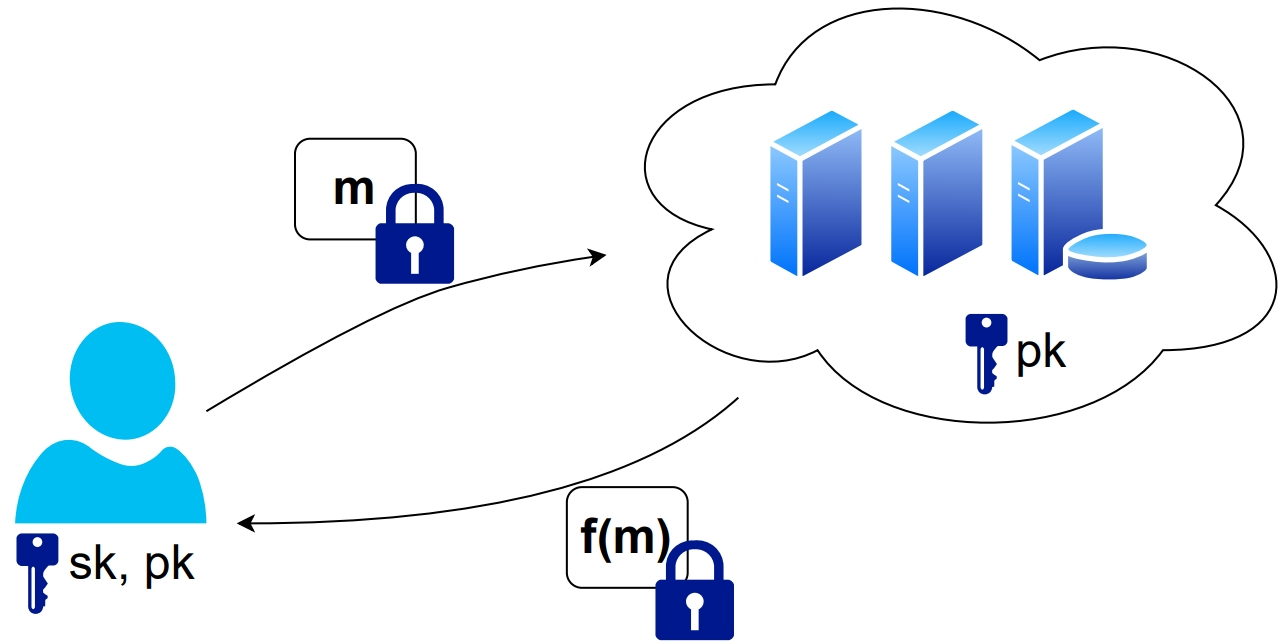
\includegraphics[scale=0.13]{fhe.jpg}
    \caption{Paper:https://ia.cr/2022/657}
    \end{figure}
    \column{0.4\textwidth}
    \begin{itemize}
        \item Client encrypted data (SK).
        \item Send data and PK to server.
        \item Server operates with out decrypt it.
        \item Server send back the result.
        \item Client decrypts the result with SK.
    \end{itemize}
\end{columns}
\pause
\pause
    \vspace{-0.2cm}
    \textbf{Present}: Orders of magnitude \textbf{slower} for real use.
\end{frame}
%%%%%%%%%%%%%%%%%%%%%%%%%%%%%%%%%%%%%%%%%%%%%%%%%%%%%%%%%%%%%%%%%%%%%%%%%%%%%%%%%%%%%%%%%%%%%%%%%%%%
% HABlar  de ckks bgv y bfv
\begin{frame}
            \frametitle{HE}
    HE supports only addition, multiplication and rotation $\rightarrow$ only \textbf{linear} operations.
\pause
    \vspace{0.3cm}
  \begin{columns}
    \column{0.5\textwidth}
      In general, HE schemes use \texttt{Ring Learning With Errors} (RLWE) that
      \textbf{adds some noise} (error) to the encryption.

\pause
\vspace{0.3cm}
      This \textbf{noise grows} in each operation (particularly with \textbf{multiplications}).

\vspace{0.3cm}
      If the noise is too big will be \textbf{undecryptable}.
\pause
    \column{0.5\textwidth}
        \begin{figure}[h!]
            \centering
            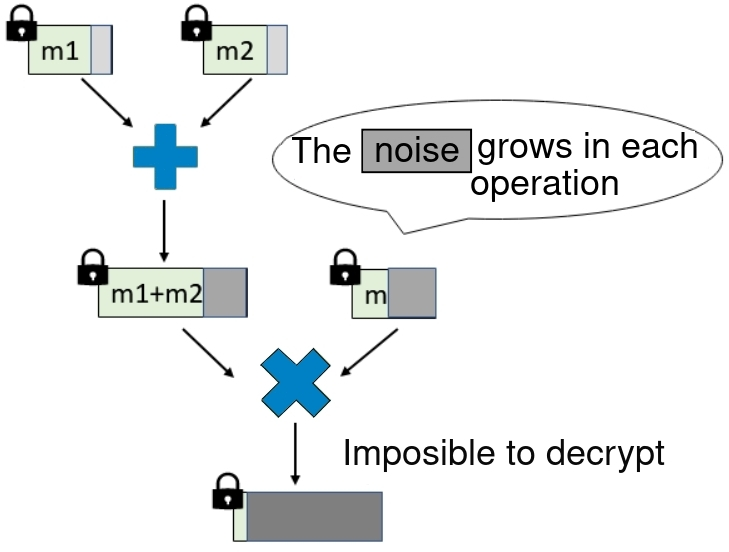
\includegraphics[scale=0.2]{multNoise.jpg}
        \end{figure}

\end{columns}

\pause
    Fully Homomorphic Encryption (FHE): \textbf{Unlimited} number of operations. In this type of schemes
    it use \texttt{Bootstrapping} that are techniques that refresh this error.

\pause
    Even slower!!!
\end{frame}


%%%%%%%%%%%%%%%%%%%%%%%%%%%%%%%%%%%%%%%%%%%%%%%%%%%%%%%%%%%%%%%%%%%%%%%%%%%%%%%%%%%%%%%%%%%%%%%%%%%%
\begin{frame}
    \frametitle{HE schemes}

Popular schemes:
 \vspace{-0.25cm}
\begin{itemize}\itemsep-0.9em
    \item Operations on integers: BFV and BGV.
    \item Operations on real numbers: CKKS.
\end{itemize}

    Amount of noise available until undecryptable (''noise budget'') parameter of scheme depence.

Generally bigger parameters bigger noise budget.

    Works in a \textbf{Polynomial Ring} domain.

%\vspace{-0.25cm}
%\textbf{Ring}: a set with addition, subtraction and multiplication. (and other property's, commutative, associative, etc).

\pause
 \vspace{-0.25cm}
    This operations of elements in a ring return elements in the ring $\rightarrow$  \textbf{modular arithmetics}.

 \vspace{-0.25cm}
\textbf{Parameters}: are application-specific and desired security.

\pause
 \vspace{-0.3cm}
\begin{itemize}\itemsep-0.9em
%    \item $\lambda$ security level. $\sim$ $2^\lambda$ operation to decrypt with prob 1. (128, 256.)
    \item $N$: the degree of the Polynomials ($N$-1):  8192, 16384, 32768.
\pause
    \item $q$ and $t$: the mod of the coefficients: $t$ << $q$ = $2^{218}$,   $2^{438}$,  $2^{881}$.
\end{itemize}
\end{frame}


%%%%%%%%%%%%%%%%%%%%%%%%%%%%%%%%%%%%%%%%%%%%%%%%%%%%%%%%%%%%%%%%%%%%%%%%%%%%%%%%%%%%%%%%%%%%%%%%%%%%
% Puede volar esta
\begin{frame}
    \frametitle{BFV Primitives}
\begin{itemize}\itemsep-0.9em
    \item ParamGen($\lambda$)$\rightarrow$ Default Params.
    \item KeyGen(Params) $\rightarrow$ SK, PK, EvalK (each is a tuple of two polynomials)
        \SubItem{ Sample 3 polynomials, two polynomial multiplication, two additions and two modulus.}
\pause
    \item Encrypt(PK, m) $\rightarrow$ c (tuple of two polynomials)
        \SubItem{ Sample 3 polynomials, two polynomial multiplication, one scalar multiplication, three additions and two modulus.}
    \item Decrypt(SK, c) $\rightarrow$ m
        \SubItem{ similar to Encryption.}
\pause
    \item EvalAdd(c$_1$, c$_2$) $\rightarrow$ c$_3$ (tuple of two polynomials)
    \item EvalMult(c$_1$, c$_2$) $\rightarrow$ c$_{mul}$ (tuple of three polynomials)
\pause
    \item Relinerize(c$_{mul}$, EvalK) $\rightarrow$ c$_{mul}$' (tuple of two polynomials)
        \SubItem{ Six polynomial multiplications, three additions and five modulus.}
\end{itemize}


\end{frame}

%%%%%%%%%%%%%%%%%%%%%%%%%%%%%%%%%%%%%%%%%%%%%%%%%%%%%%%%%%%%%%%%%%%%%%%%%%%%%%%%%%%%%%%%%%%%%%%%%%%%
\section{Future Work}
\begin{frame}
    \frametitle{SEAL profile}
Microsft SEAL: HE library.
    \begin{figure}
        \begin{minipage}[c]{0.49\linewidth}
            \includegraphics[width=\linewidth]{ckks_N.png}
            \caption{Execution time and memory usage to compute $X^2$ (element-wise) using CKKS for different polynomial ring degrees $N$.}
        \end{minipage}
        \hfill
        \begin{minipage}[c]{0.49\linewidth}
            \includegraphics[width=\linewidth]{ckks_mult_depth.png}
            \caption{ Consumption time and memory usage for computing different powers of a vector in CKKS scheme for the polynomial ring degree $N=32768$.
    In the left side its shows the time y-axis and in the right side the memory y-axis.
}
        \end{minipage}%
    \end{figure}
\end{frame}
%%%%%%%%%%%%%%%%%%%%%%%%%%%%%%%%%%%%%%%%%%%%%%%%%%%%%%%%%%%%%%%%%%%%%%%%%%%%%%%%%%%%%%%%%%%%%%%%%%%%
\begin{frame}
    \frametitle{Bit error}

\end{frame}
%%%%%%%%%%%%%%%%%%%%%%%%%%%%%%%%%%%%%%%%%%%%%%%%%%%%%%%%%%%%%%%%%%%%%%%%%%%%%%%%%%%%%%%%%%%%%%%%%%%%
\begin{frame}
    \frametitle{CKKS vs BFV/BGV}
    \begin{figure}
        \begin{minipage}[c]{0.49\linewidth}
            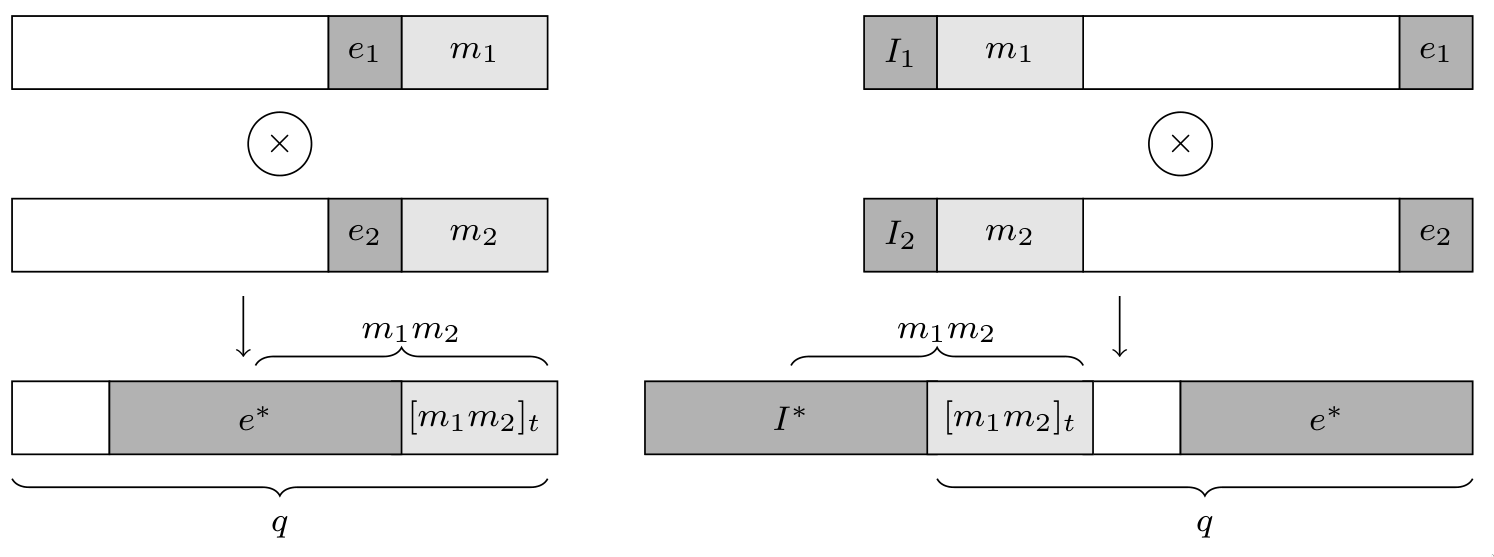
\includegraphics[width=\linewidth]{encoding.png}
            \caption{Image A}
        \end{minipage}
        \hfill
        \begin{minipage}[c]{0.49\linewidth}
            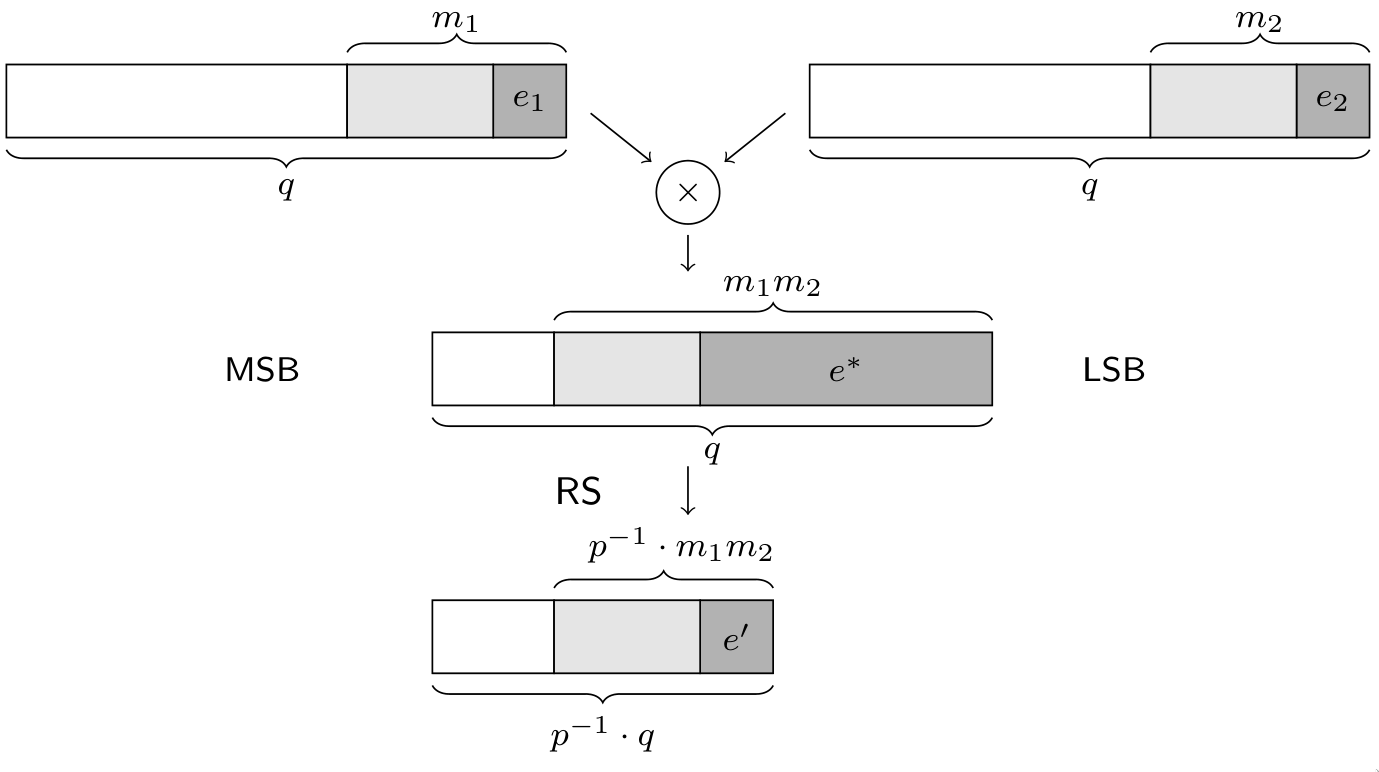
\includegraphics[width=\linewidth]{encoding-ckks.png}
            \caption{Image B}
        \end{minipage}%
    \end{figure}
\end{frame}
%%%%%%%%%%%%%%%%%%%%%%%%%%%%%%%%%%%%%%%%%%%%%%%%%%%%%%%%%%%%%%%%%%%%%%%%%%%%%%%%%%%%%%%%%%%%%%%%%%%%
\section{Conclusion}
\begin{frame}
    \frametitle{Conclusion}
    Conclusion
\end{frame}

%%%%%%%%%%%%%%%%%%%%%%%%%%%%%%%%%%%%%%%%%%%%%%%%%%%%%%%%%%%%%%%%%%%%%%%%%%%%%%%%%%%%%%%%%%%%%%%%%%%%
\begin{frame}[noframenumbering]
\frametitle{}

\end{frame}
%%%%%%%%%%%%%%%%%%%%%%%%%%%%%%%%%%%%%%%%%%%%%%%%%%%%%%%%%%%%%%%%%%%%%%%%%%%%%%%%%%%%%%%%%%%%%%%%%%%%
\end{document}
